\documentclass[conference]{IEEEtran}
\IEEEoverridecommandlockouts
% The preceding line is only needed to identify funding in the first footnote. If that is unneeded, please comment it out.
\usepackage{cite}
\usepackage{amsmath,amssymb,amsfonts}
\usepackage{algorithmic}
\usepackage{graphicx}
\usepackage{textcomp}
\usepackage{xcolor}
\usepackage{url}
\usepackage{hyperref}
\usepackage{float}
\usepackage{moresize}
\usepackage{booktabs}
\usepackage[para,online,flushleft]{threeparttable}


\makeatletter
\newcommand{\linebreakand}{%
  \end{@IEEEauthorhalign}
  \hfill\mbox{}\par
  \mbox{}\hfill\begin{@IEEEauthorhalign}
}
\makeatother



\def\BibTeX{{\rm B\kern-.05em{\sc i\kern-.025em b}\kern-.08em
    T\kern-.1667em\lower.7ex\hbox{E}\kern-.125emX}}
\begin{document}

\title{Profundizando el análisis de \textit{CheMarket Inc.}}

\author{%
\IEEEauthorblockN{Adrián Arturo Suárez García}
\IEEEauthorblockA{202123771\\
\href{mailto:a.suarezg@uniandes.edu.co}{\texttt{a.suarezg@uniandes.edu.co}}}
\and
\IEEEauthorblockN{Luis Alejandro Rubiano Guerrero}
\IEEEauthorblockA{202013482\\
\href{mailto:la.rubiano@uniandes.edu.co}{\texttt{la.rubiano@uniandes.edu.co}}}
\and
\IEEEauthorblockN{Gabriel Alejandro Moreno Riveros}
\IEEEauthorblockA{202014583\\
\href{mailto:g.morenor@uniandes.edu.co}{\texttt{g.morenor@uniandes.edu.co}}}
\linebreakand
\IEEEauthorblockN{Gianluca Cicco}
\IEEEauthorblockA{202020881\\
\href{mailto:g.cicco@uniandes.edu.co}{\texttt{g.cicco@uniandes.edu.co}}}
\and
\IEEEauthorblockN{Juan Sebastián Sierra}
\IEEEauthorblockA{202020881\\
\href{mailto:j.sierrat@uniandes.edu.co}{\texttt{j.sierrat@uniandes.edu.co}}}
}



\maketitle


\section{Introducción}
A través de este informe, nuestro grupo de economistas y científicos de datos emplea nuevas técnicas de análisis estadístico y de machine learning para 
descubrir relaciones no lineales y efectos heterogéneos en el comportamiento de los usuarios en \textbf{CheMarket Inc.} En particular, nos enfocamos en entender qué variables impulsan el revenue de la compañía, con el fin de generar evidencia que apoye la toma de decisiones estratégicas informadas.

\section{Datos observacionales: ¿Qué impulsa las ventas?}

\subsection{Datos y preparación}

Para el análisis observacional, al igual que en nuestro primer informe contamos con un conjunto de $100.000$ observaciones históricas de los usuarios de CheMarket. Las variables disponibles son $\texttt{time\_spent}$: tiempo en el sitio durante la sesión, $\texttt{past\_sessions}$: número de sesiones anteriores, 
$\texttt{device\_type}$: tipo de dispositivo (móvil, escritorio, tablet), $\texttt{os\_type}$: sistema operativo (OS X, Windows, otros), $\texttt{is\_returning\_user}$: si el usuario ya había visitado antes, $\texttt{sign\_up}$: si se registró o no y $\texttt{revenue}$: cuanto gastó en cada sesión.

En la siguiente tabla se presentan las estadísticas descriptivas de estas variables.


\begin{table}[H]
\tiny
\centering
\caption{Estadísticas descriptivas de las variables}
\begin{tabular}{|l|c|c|c|c|c|c|}
\hline
 & \textbf{Tiempo} & \textbf{Sesiones} & \textbf{Dispositivo} & \textbf{OS} & \textbf{Recurrente?} & \textbf{Revenue} \\
\hline
Mín & 0.000125 & 0 & Tablet: 9882 & Otro: 9909 & No: 4930 & 0.5451 \\
25\% & 1.4247 & 2 & Escritorio: 40009 & OS X: 30253 & Sí: 95070 & 2.3400 \\
Mediana & 3.4384 & 3 & Móvil: 50109 & Windows: 59838 & & 3.1370 \\
50\% & 4.9946 & 3.001 & & & & 3.9766 \\
75\%  & 6.9117 & 4  & & & & 4.5221 \\
Máx & 54.3989 & 14  & & & & 36.2934 \\
\hline
\end{tabular}

\hfill \break
Estadísticas descriptivas de las variables numéricas y cantidad por clase para las categóricas.

\end{table}

Aquí dividimos la base en entrenamiento (70\%) y validación (30\%) y transformamos la variable objetivo a logartimico (log\_revenue) para estabilizar la dispersión. Luego, enumeramos todas las variables que el modelo puede usar y, en algunos casos incluimos transformaciones simples o interacciones como en nuestro primer informe. 


\subsection{Regresiones Lineales}

Vamos a evaluar, un modelo lineal clásico (OLS) y para mejorar la predicción y evitar posibles sobreajustes, usamos además dos variantes: Ridge y Lasso.  Ambos agregan un término de penalización. Ridge añade una penalización L2 (cuadrada) a la magnitud de los coeficientes, mientras Lasso usa una penalización L1 (valor absoluto). Para elegir la fuerza de esa penalización (el hiperparámetro $\lambda$) utilizamos validación cruzada en datos de entrenamiento. Entonces seleccionamos dos candidatos: $\lambda_{min}$, que minimiza el MSE medio, y además $\lambda_{1se}$, que es el valor más grande de $\lambda$ cuyo error sigue estando dentro de una desviación estándar del mínimo, pues permite escoger el modelo más sencillo (menor sobreajuste) sin sacarificar en gran medida la exactitud.


\begin{table}[H]
\caption{Comparación de modelos predictivos}
\centering
\begin{tabular}[t]{l|l|l|l}
\hline
Modelo & MSE & RMSE & R²\\
\hline
LM Básico & 0.2840 & 0.5329 & 0.0057\\
\hline
LM Todas & 0.1985 & 0.4455 & 0.3050\\
\hline
LM Interacciones & 0.1983 & 0.4453 & 0.3058\\
\hline
Ridge ($\lambda_{min}$) & 0.1984 & 0.4455
($\lambda = 0.025197$) & 0.3051\\
\hline
Ridge ($\lambda_{1se}$) & 0.1991 & 0.4462
($\lambda = 0.058207$) & 0.3030\\
\hline
Lasso ($\lambda_{min}$) & 0.1983 & 0.4453
($\lambda = 0.000311$) & 0.3058\\
\hline
Lasso ($\lambda_{1se}$) & 0.1987 & 0.4457
($\lambda = 0.008847$) & 0.3043\\
\end{tabular}
\end{table}

La Tabla II muestra primero que el LM Básico rinde claramente peor, lo que confirma que el gasto es fuertemente condicional en las otras variables. Al incluir covariables (tiempo en el sitio transformado, sesiones previas, dispositivo, usuario recurrente y sistema operativo), el desempeño mejora sustancialmente y LM Interacciones apenas mejora un poco más. Cuando pasamos a Ridge y Lasso, los resultados quedan prácticamente empatados con LM Interacciones (MSE/RMSE bastante similares). Estas relaciones se deben a que con pocas variables y relaciones bastante lineales, OLS ya capta todo el efecto y la regularización no mejora mucho la predicción fuera de muestra.

\subsection{Árboles de Clasificación y Regresión (CART)}

Si nos basamos en lo anterior, sabemos las regresiones lineales (OLS, Ridge y Lasso) ofrecían desempeños muy parecidos. Por lo tanto, si queremos evaluar posibles mejoras en el MSE/RMSE es pertinente evaluar patrones no lineales e interacciones que modelos lineales no identifican de manera apropiada. En este orden de ideas, vamos a comprobar si un árbol de regresión (CART) mejora la predicción fuera de muestra y, de paso, ofrece reglas que nos ayuden a entender subgrupos de usuarios con niveles de gasto distinto.

\hfill \break

\subsubsection{Profundidad por Iteraciones}

\subsection{Recomendación preliminar}


En este caso, vamos a entrenar un CART de regresión, usando validación cruzada y un rango de profundidades $(1,\dots,10)$, en donde iterativamente vamos a generar un arbol para cada profundidad dentro del rango y luego calculamos el error de validación promedio; escogemos la profundidad con mejor desempeño y en cada iteración elige la variable que más reduce el error dentro de las ramas. Puesto que, la profundidad en un arbol controla la complejidad del modelo; arboles más profundos capturan más detalles, pero pueden sobreajustar; arboles menos profundos generalizan mejor pero pueden quedarse cortos. Con validación cruzada buscamos un punto intermedio que mejor predice fuera de muestra. Con nuestros datos, el optimo fue 4. 
En la siguiente figura se muestra este arbol con sus subgrupos de decisión.

\begin{figure}[h]
    \centering
    \includegraphics[width=0.5\textwidth]{figures/arbol\_profundidad.png}
    \caption{Árbol de regresión con profundidad 4}
    \label{fig:arbol_profundidad}
\end{figure}

Viendo el arbol, se ve que el primer nodo aparece la raíz del tiempo con un umbral cercano a 2.2. Al estar en la parte superior, indica que para predecir el gasto, el modelo primero separa a los usuarios
 según su tiempo en el sitio. Además, la relación no es lineal: a mayor tiempo en el sitio, mayor es el efecto sobre el gasto. Si vemos la rama izquierda, para los usuarios de poco tiempo en el sitio,
  el tipo de dispositivo ayuda mucho a distinguir el gasto esperado. Eso quiere decir, que los usuarios de paso rápido no se comportan igual en móvil que en desktop/Tablet. Por otro lado, la rama derecha, exhibe que para las personas que pasan mas tiempo en sitio, el historial de sesiones marca claras diferencias en el gasto.
   Para los usuarios con el mayor número de sesiones previas ($>4$), conviene distinguir entre sistema operativo (os\_type), y es evidente que conviene optimizar la experiencia para dispositivo con Os, pues tienen el mayor gasto esperado en este nodo.

  \subsubsection{Pruning (poda) para profundidad}

  A diferencia del método anterior, en donde controlando ex ante su tamaño, vamos a dejar el árbol completo y luego lo vamos a ir simplificando mediante pruning (poda) para evitar sobreajuste. Para ello definimos la ecuacion de costo de complejidad:
 $C_{\alpha}(T) = \text{Error}(T) + \alpha |T|$.

Donde \textit{Error}(T) resume el error cuadrático en las hojas y 
$|T|$ es cuántas hojas usamos.

El parámetro $\alpha$ (cp) es la penalización por complejidad, que funciona como un umbral mínimo de mejora en el error; cada posible división se acepta solo si reduce el error de predicción en más de cp; de lo contrario, esa rama se elimina. La idea, es ir podando con un cp fijo hasta encontrar el arbol que optimiza el costo de complejidad.

No obstante, para determinar este hiperparametro(cp) utilizamos validación cruzada 10-fold y con un rango de valores ( de $0.00001$ a $0.0001$). Probamos todos esos valores de cp, y nos quedamos con el que mejor predice fuera de muestra.

\begin{figure}[h]
    \centering
    \includegraphics[width=0.5\textwidth]{figures/arbol\_complejidad.png}
    \caption{Árbol de regresión con pruning por complejidad}
    \label{fig:arbol_complejidad}

\end{figure}


Como en el árbol previo, la primera división está en la variable sqrt\_time\_spent, confirmando que el tiempo en el sitio es el predictor más relevante. A partir de ahí, el árbol sigue manteniendo la jerarquía global de manera general ( Tiempo – Sesiones - Dispositivos/OS), lo cual implica consistencia entre los métodos para plantear las  políticas. Sin embargo, a diferencia del método anterior, el pruning por complejidad recorta las divisiones que no mejoran la predicción y permite mayor complejidad donde si es necesario. De ahí que, el arbol queda mas profundo(Depth=6) donde la adición de esta variable si mejora la predicción del modelo. De ahí que, a gente que pasa más tiempo en el sitio y acumula más sesiones ($\geq 4$), no solo conviene distinguir entre sistema operativo (os\_type) sino que también importa el tipo de dispositivo (device\_type); dentro de este grupo también conviene distinguir según móvil o desktop ,lo cual es crucial porque en esas ramas están los usuarios con mayor gasto esperado Pero si el grupo, debería enfocarse en un solo grupo, debería ser los usuarios que pasen mas tiempo en sitio y  acumulan mas de 4 sesiones y que tengas sistema operativo OSX (predicción mas alta de gasto 2.48)

\subsubsection{Analisis conjunto}


\begin{table}[H]
\caption{Comparación de modelos predictivos}
\centering
\begin{tabular}[t]{l|l|l|l}
\hline
Modelo & MSE & RMSE & R²\\
\hline
LM Básico & 0.2840 & 0.5329 & 0.0057\\
\hline
LM Todas & 0.1985 & 0.4455 & 0.3050\\
\hline
LM Interacciones & 0.1983 & 0.4453 & 0.3058\\
\hline
Ridge ($\lambda_{min}$) & 0.1984 & 0.4455
($\lambda = 0.025197$) & 0.3051\\
\hline
Ridge ($\lambda_{1se}$) & 0.1991 & 0.4462
($\lambda = 0.058207$) & 0.3030\\
\hline
Lasso ($\lambda_{min}$) & 0.1983 & 0.4453
($\lambda = 0.000311$) & 0.3058\\
\hline
Lasso ($\lambda_{1se}$) & 0.1987 & 0.4457
($\lambda = 0.008847$) & 0.3043\\
\hline
Árbol (Profundidad) & 0.1256 & 0.3544
(maxdepth = 5) & 0.5602\\
\hline
Árbol (Complejidad) & 0.1228 & 0.3504
(cp = 0.000060) & 0.5701\\
\hline
\end{tabular}
\end{table}


Viendo la tabla comparativa, el mejor desempeño predictivo lo entrega el árbol con poda por complejidad (cp alrededor de  0.000060) con MSE = 0.1228, RMSE = 0.3504 seguido muy de cerca por el árbol optimizado por profundidad (maxdepth = 5) con MSE = 0.1256 y  RMSE = 0.3544 . Esta caída del error fuera de muestra a comparación de los modelos lineales, confirma que en nuestros datos había no linealidades y umbrales (tiempo en el sitio, 3 y 4 sesiones, OS/dispositivo) que la forma lineal no capturaba; el árbol, en cambio, las traduce en reglas por segmentos y por eso predice mejor.


\section{Datos experimentales: ¿Funciona facilitar el registro?}

En esta segunda parte evaluamos el efecto causal de facilitar el registro (sign\_up) sobre el gasto de los usuarios de CheMarket Inc., aprovechando el diseño experimental de la base de datos.
Nuestro objetivo es estimar el impacto promedio y explorar heterogeneidad de efectos entre distintos perfiles de usuario.

\subsection{Datos y preparación}

Partimos de la misma base experimental usada en el Taller 1, con 10,000 observaciones y variables:
sign\_up (tratamiento), time\_spent, past\_sessions, device\_type, os\_type, is\_returning\_user y revenue.
Transformamos la variable de resultado a logaritmo natural (ln\_revenue) para estabilizar la varianza.


\subsection{Efecto promedio del tratamiento}

Primero estimamos el efecto medio de sign\_up mediante regresiones OLS:

\begin{itemize}
  \item Modelo Base: solo incluye la variable de tratamiento.
  \item Modelo Completo: agrega todos los controles (tiempo, sesiones, dispositivo, sistema operativo, usuario recurrente).
  \item Modelos con interacciones: permiten que el efecto de sign\_up varíe con las características tecnológicas y de comportamiento.
\end{itemize}

Esta tabla se encuentra al final.

El efecto promedio de sign\_up resulta muy pequeño y no significativo en los modelos básicos (0.013 en el modelo base y 0.001 en el completo). Sin embargo, al incluir interacciones, el coeficiente principal se eleva (0.236–0.394) pero acompañado de efectos diferenciales. En particular, los usuarios que acceden desde dispositivo móvil o emplean el sistema Windows/Other presentan interacciones negativas y significativas, lo que atenúa el impacto general. En contraste, ser un usuario recurrente amplifica notablemente el efecto (0.167 \*\*\*). Esta heterogeneidad se refleja también en la capacidad explicativa del modelo, que aumenta de un $R^2$ cercano a 0.0 hasta aproximadamente 0.35, confirmando que las diferencias entre grupos son clave para entender la respuesta observada.


\subsection{Heterogeneidad: Árbol Causal}

Para identificar subgrupos de usuarios con efectos distintos, aplicamos un honest causal tree.
El árbol divide la población según umbrales en time\_spent y past\_sessions, y según combinaciones de device\_type y os\_type.

\begin{figure}[h]
    \centering
    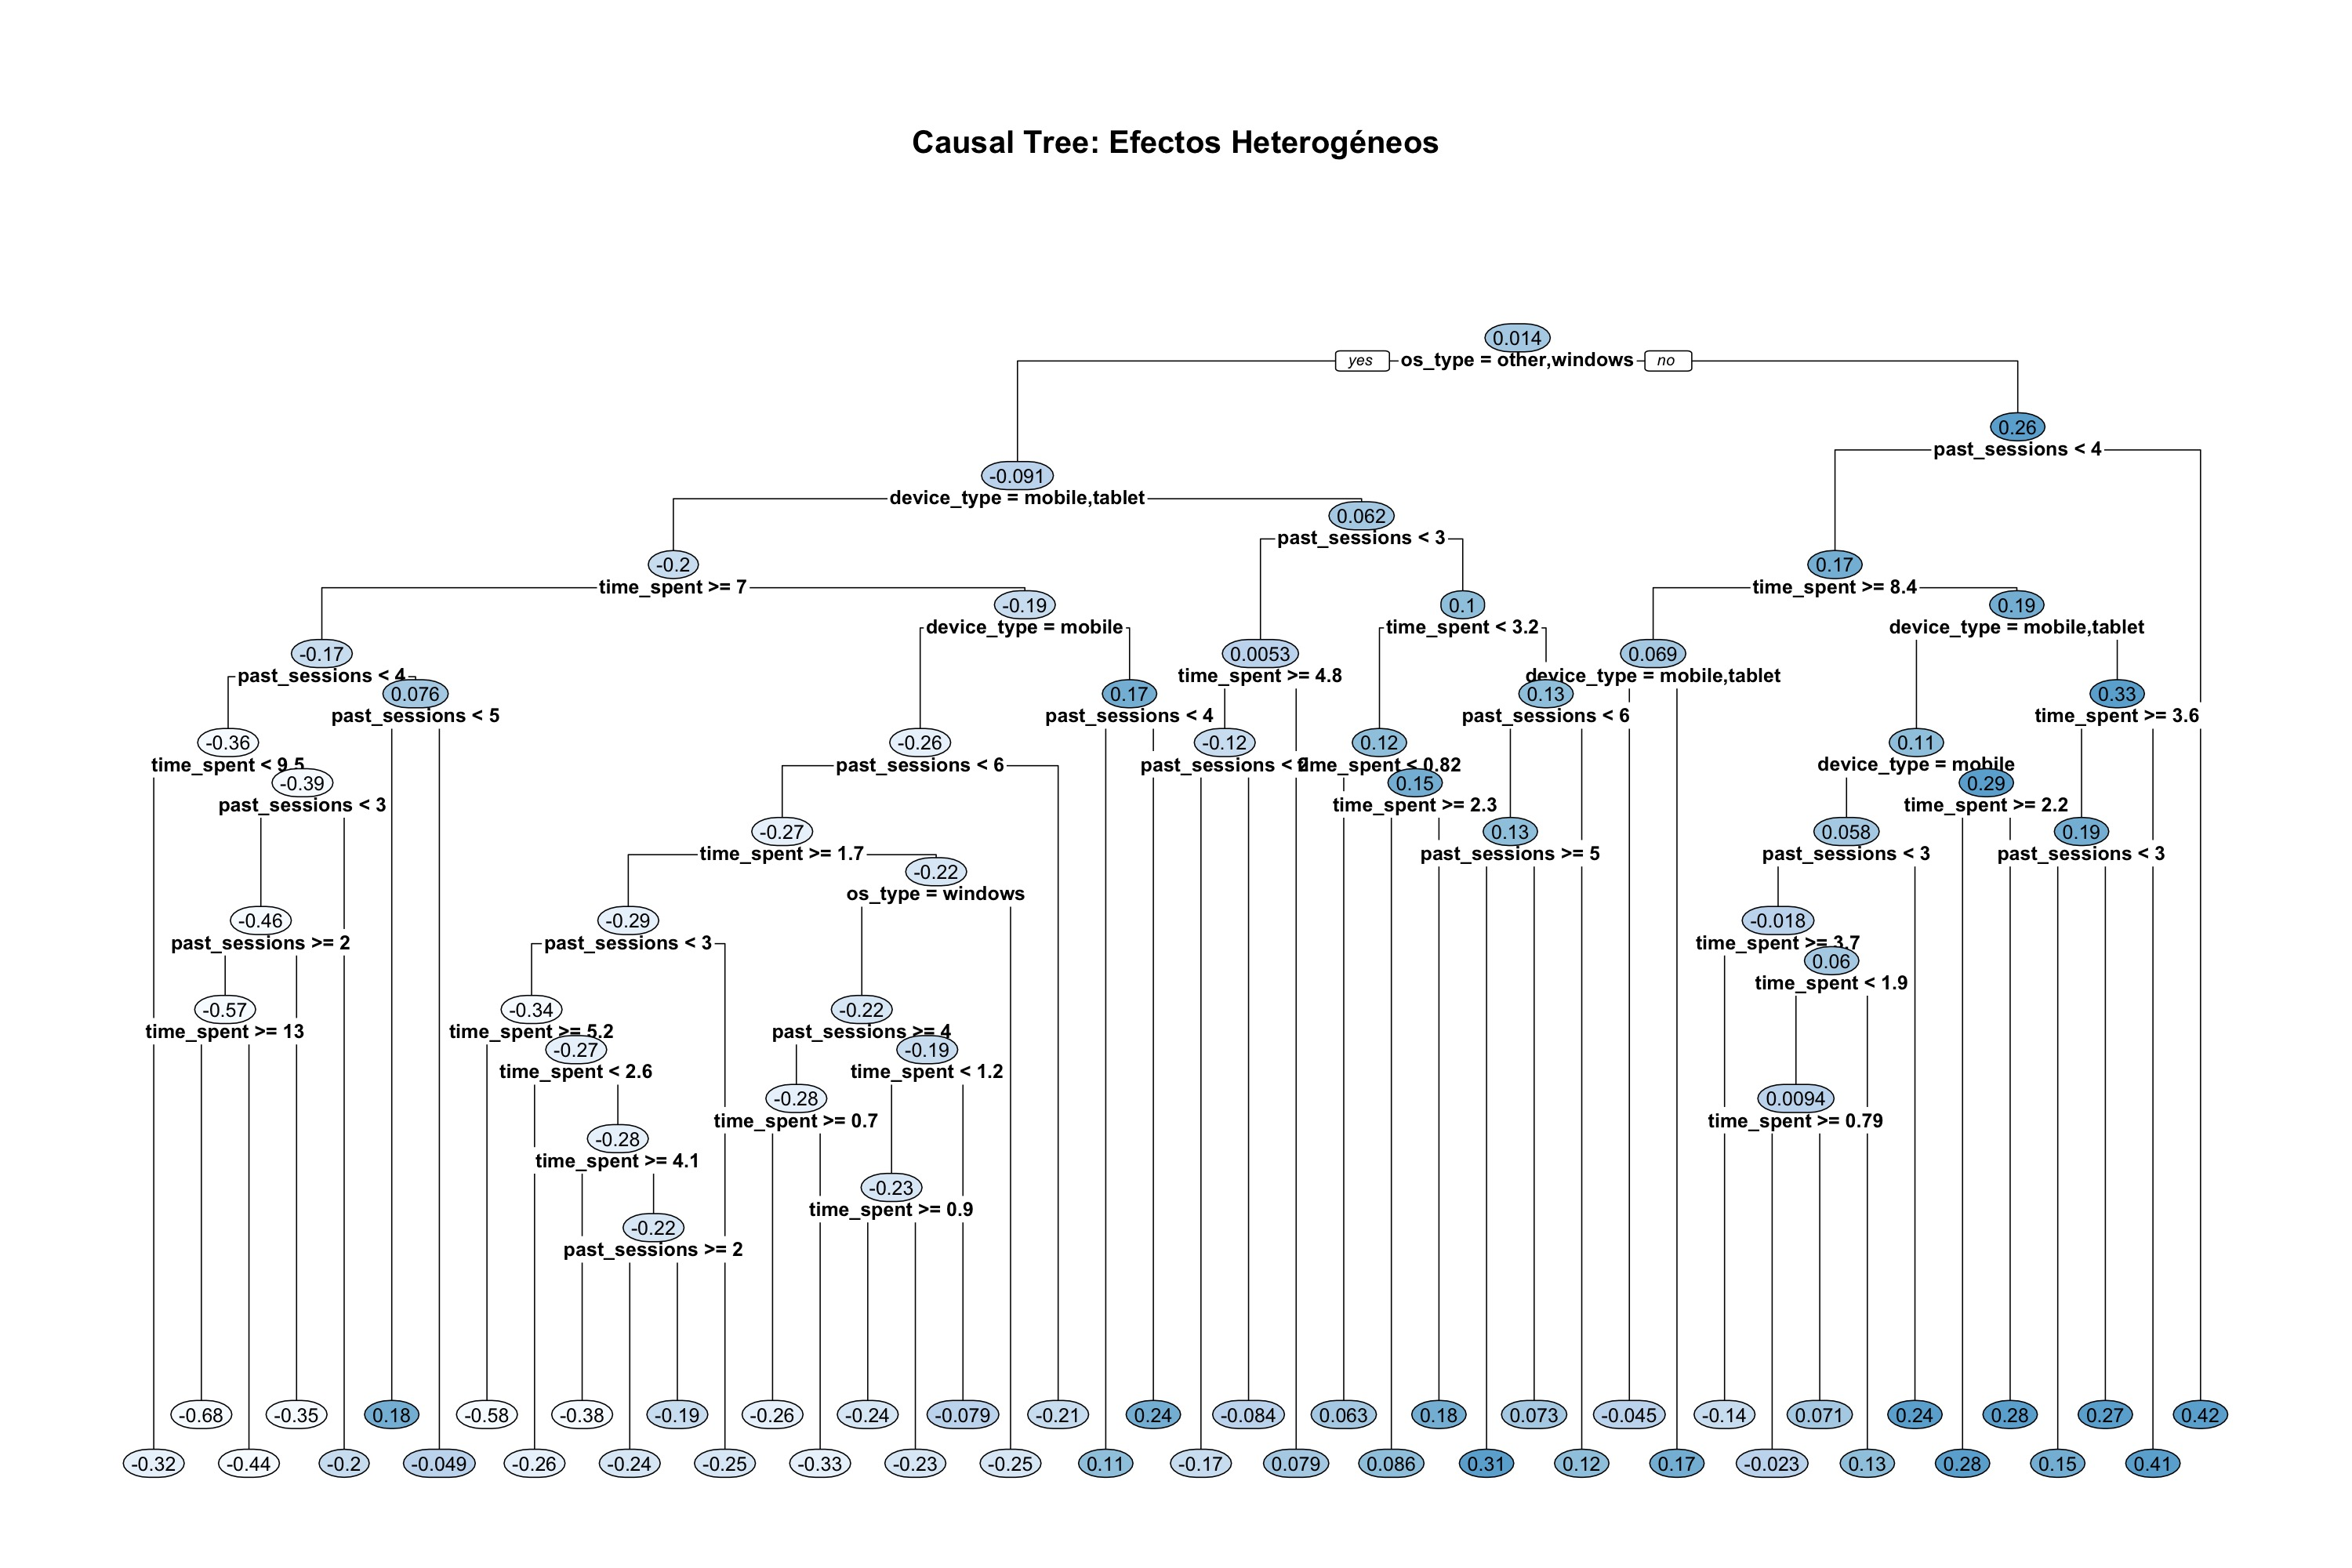
\includegraphics[width=0.5\textwidth]{figures/causal_tree_unpruned.jpg}
    \caption{Árbol Causal de Efectos Heterogéneos del Registro}
    \label{fig:arbol_causal}
\end{figure}

Principales hallazgos del árbol:

\begin{itemize}
  \item Los nodos iniciales separan a los usuarios por tiempo en sesión y número de sesiones previas, confirmando su importancia.
  \item Se observan hojas con efectos positivos de hasta $\approx 0.4$ (usuarios con tiempo largo y varias sesiones, sobre todo en OS X) y otras con efectos negativos (usuarios móviles con pocas sesiones).
  \item Esto sugiere que conviene focalizar el incentivo de registro en usuarios con mayor engagement y dispositivos de escritorio/OS X.
\end{itemize}


\subsection{Bosque Causal y CATEs}

\begin{figure}
    \centering
    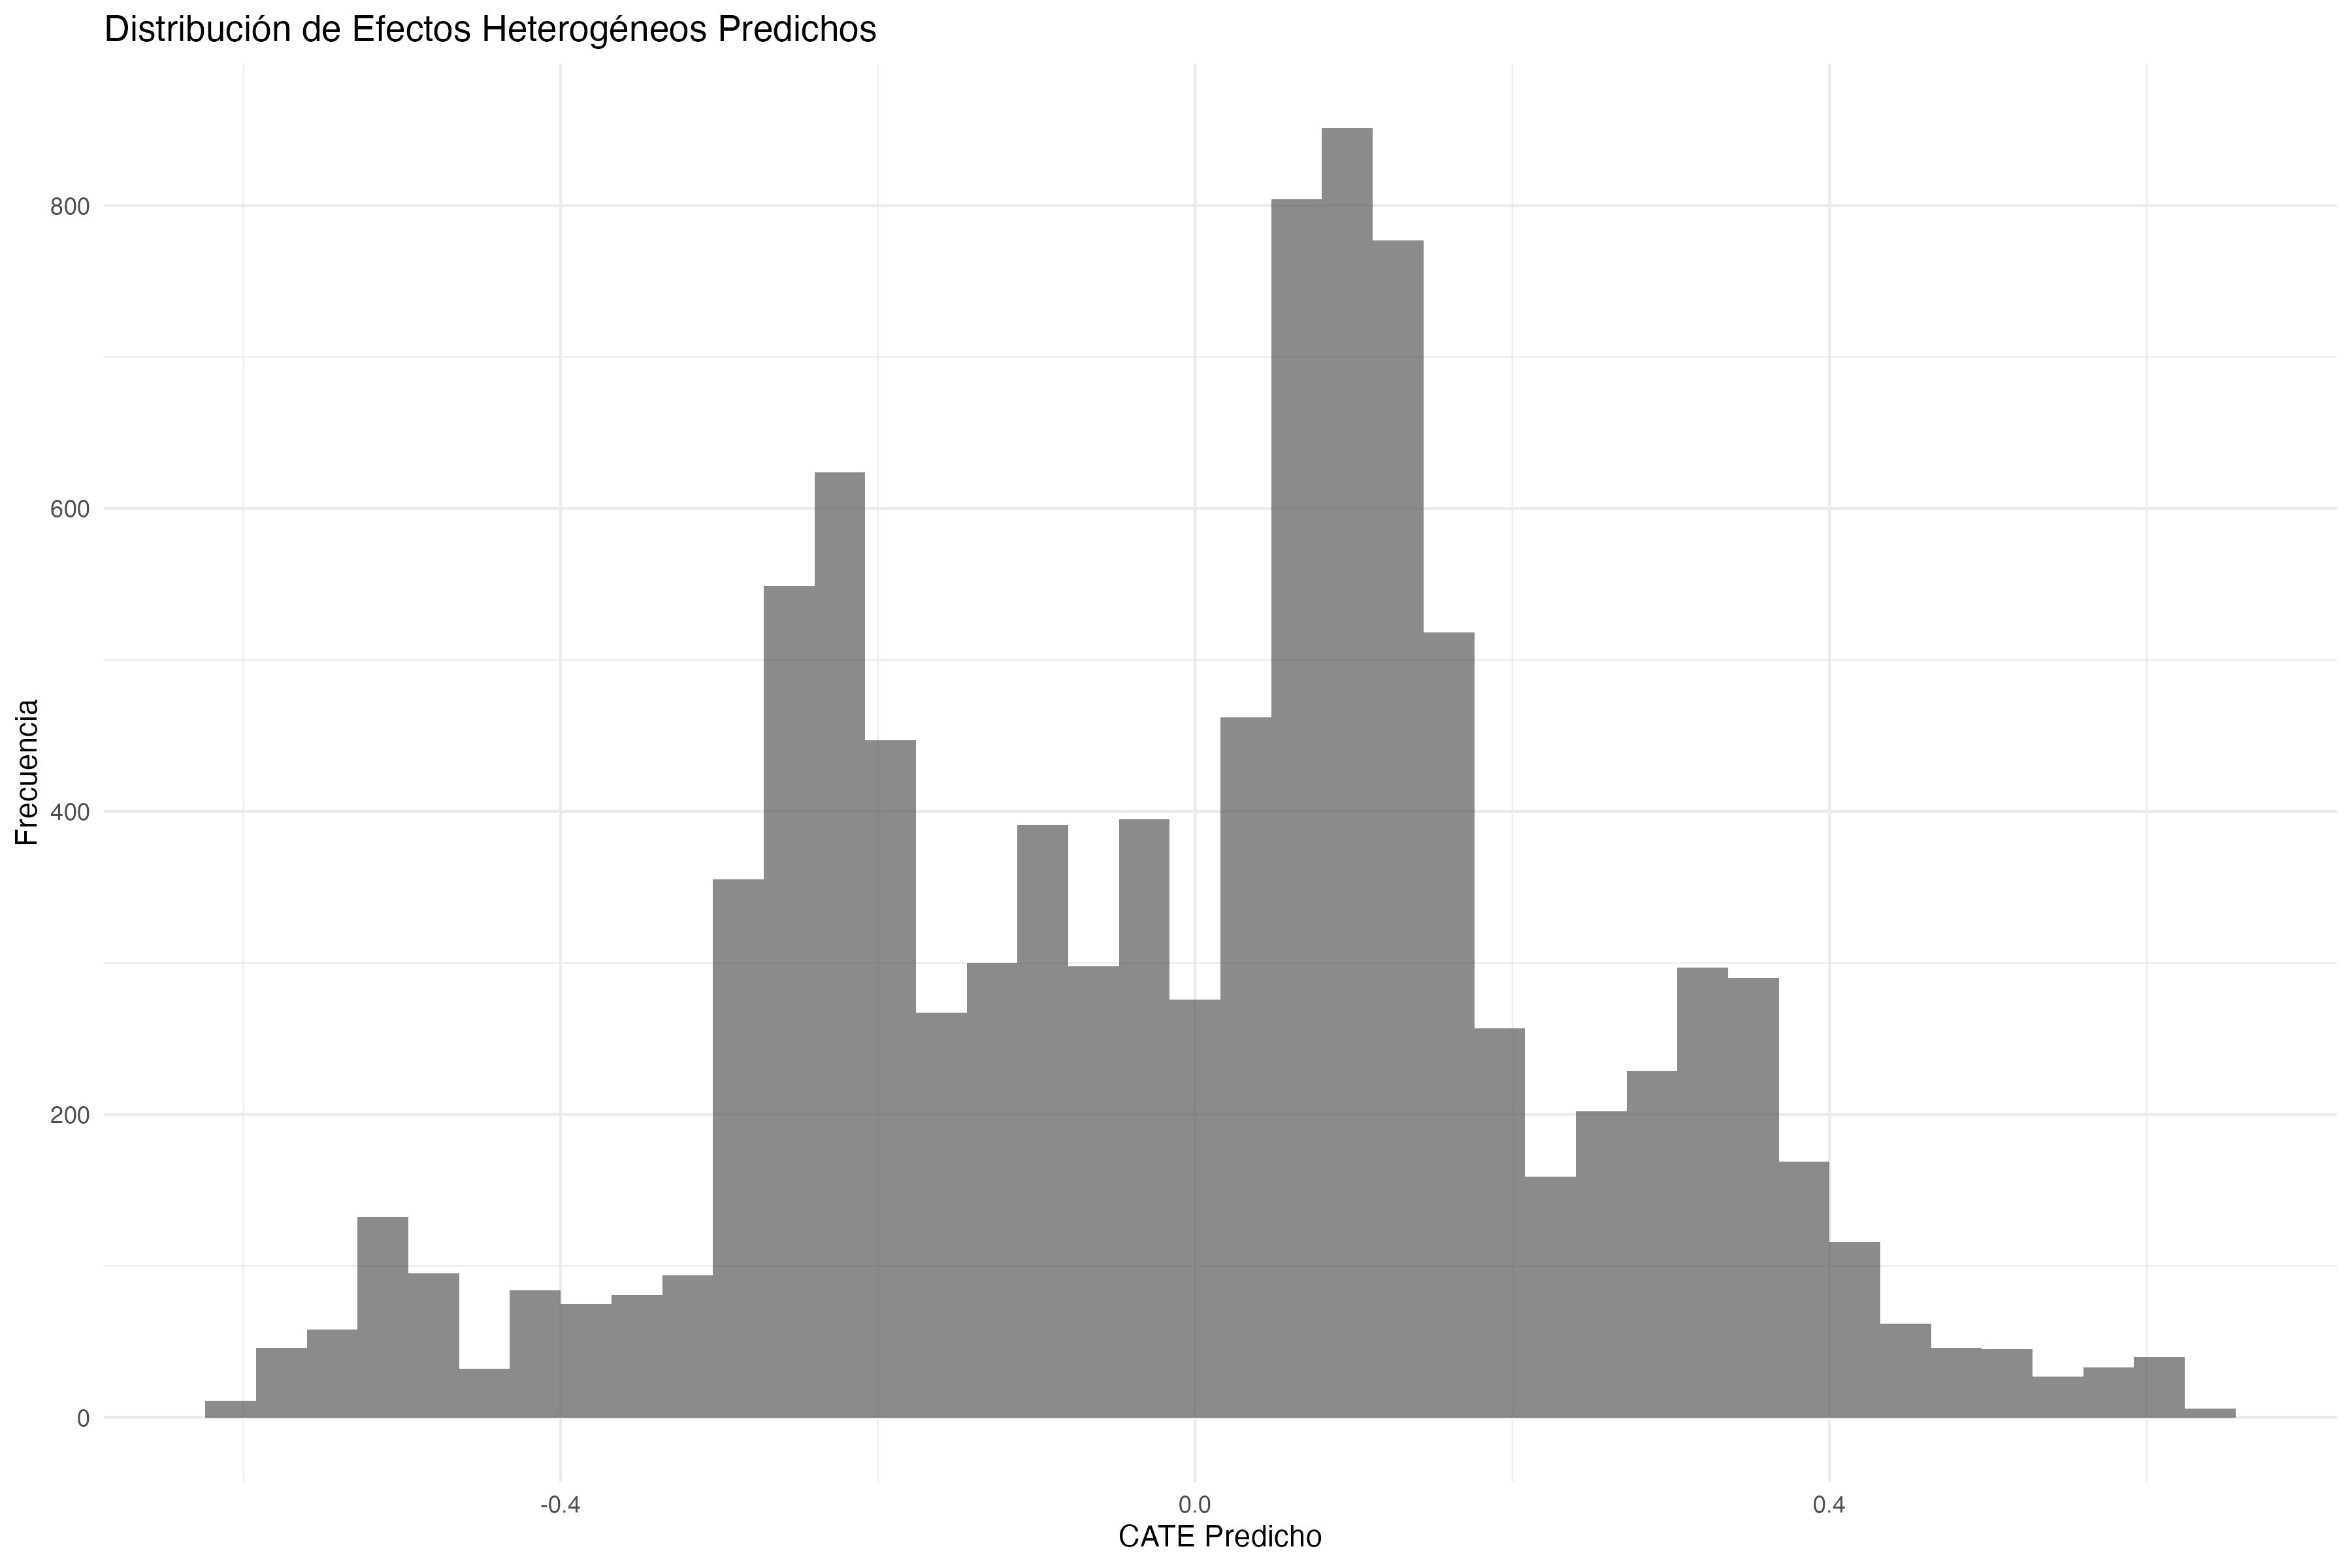
\includegraphics[width=0.3\textwidth]{figures/distribucion_efectos_heterogeneos.jpg}
    \caption{Distribución de CATEs del Registro}
    \label{fig:cate_distribution}
\end{figure}

Para robustecer los resultados usamos un causal forest (grf) con 10000 árboles, que permite estimar el efecto de tratamiento condicional (CATE) para cada observación.

Los CATEs confirman una distribución amplia:
hay usuarios con efectos cercanos a cero, otros claramente positivos ($>0.3$) y un grupo minoritario con efectos negativos ($<–0.2$).

\subsection{Visualización de patrones de heterogeneidad}

A continuación mostramos algunos cruces clave:

\subsection{Discusión y recomendaciones}

La evidencia experimental muestra que el efecto promedio de facilitar el registro sobre el gasto es bajo y poco significativo, pero esconde una heterogeneidad marcada. Los usuarios que combinan sistema operativo OS X, dispositivo de escritorio o tablet, varias sesiones previas y tiempos prolongados en el sitio presentan CATEs claramente positivos, mientras que usuarios móviles con pocas sesiones y sistemas Windows u “other” exhiben efectos nulos o incluso negativos. En conjunto, estos resultados sugieren que una política uniforme de incentivos al registro sería ineficiente; en su lugar, conviene focalizar la intervención en los segmentos de alto potencial, donde el beneficio económico de promover el registro es más alto y más seguro.



\begin{table}[H]
\tiny
\centering
\caption{Efectos del Registro en el Ingreso de CheMarket}
\label{tab:efectos_registro}
\begin{threeparttable}
\begin{tabular}{lcccc}
\toprule
 & \multicolumn{4}{c}{\textbf{Dependent variable: Log(Gasto Mensual)}} \\
\cmidrule(lr){2-5}
 & Modelo Base (1) & Modelo Completo (2) & Modelo Efectos Heterogéneos (1) (3) & Modelo Efectos Heterogéneos (2) (4) \\
\midrule
Tratamiento (Registro)      & 0.013 & 0.001 & 0.394** & 0.236** \\
                            & (0.012) & (0.010) & (0.021) & (0.046) \\
Tiempo                      & 0.048** & 0.048* & 0.048* & 0.048** \\
                            & (0.001) & (0.001) & (0.001) & (0.001) \\
Sesiones Pasadas            & 0.099** & 0.099* & 0.099* & 0.099** \\
                            & (0.003) & (0.003) & (0.003) & (0.003) \\
Dispositivo: Móvil          & -0.326** & -0.171* & -0.171** \\
                            & (0.010) & (0.014) & (0.014) \\
Dispositivo: Tablet         & -0.072** & -0.076* & -0.076** \\
                            & (0.018) & (0.024) & (0.024) \\
Sistema: Otro               & -0.186*** & -0.001 & -0.0005 \\
                            & (0.018) & (0.025) & (0.025) \\
Sistema: Windows            & -0.190*** & -0.021 & -0.021 \\
                            & (0.011) & (0.015) & (0.015) \\
Usuario Recurrente          & -0.098** & -0.095* & -0.179** \\
                            & (0.024) & (0.024) & (0.032) \\
Registro: Móvil             &         & -0.308** & -0.309** \\
                            &         & (0.020) & (0.020) \\
Registro: Tablet            &         & 0.011 & 0.011 \\
                            &         & (0.034) & (0.034) \\
Registro: Sistema Otro      &         & -0.372** & -0.375** \\
                            &         & (0.035) & (0.035) \\
Registro: Sistema Windows   &         & -0.339** & -0.340** \\
                            &         & (0.022) & (0.022) \\
Registro: Usuario Recurrente &        &         & 0.167*** \\
                            &         &         & (0.043) \\
Constante                   & 1.222** & 1.084* & 0.884* & 0.964** \\
                            & (0.008) & (0.025) & (0.026) & (0.033) \\
\midrule
Observations                & 10,000 & 10,000 & 10,000 & 10,000 \\
R$^{2}$                     & 0.0001 & 0.318 & 0.352 & 0.353 \\
Adjusted R$^{2}$            & 0.00003 & 0.317 & 0.352 & 0.352 \\
Residual Std. Error         & 0.599 (df = 9998) & 0.495 (df = 9991) & 0.482 (df = 9987) & 0.482 (df = 9986) \\
F Statistic                 & 1.253 (df = 1; 9998) & 581.899** (df = 8; 9991) & 452.654* (df = 12; 9987) & 419.553** (df = 13; 9986) \\
\bottomrule
\end{tabular}
\begin{tablenotes}
\small
\item \textit{Note}: Errores estándar en paréntesis. * p$<$0.01, ** p$<$0.05, * p$<$0.1.
\end{tablenotes}
\end{threeparttable}
\end{table}




\end{document}
